\section{Problem 2C: Stochastic SEIIaR model}

\subsection{a)}

The time-development of all the variables in the SEIIaR model is shown in figure \ref{fig:SEIIaR}, showing $10$ realisations of the simulation. The continuous lines shows the solutions of the deterministic model. To compare it easily with the deterministic model, we contract $E,I,I_a$ into one variable, so that they together represent all the infected people. The solutions of the deterministic model are shown together with the contracted versions of these simulations in figure \ref{fig:SEIIaR_compare}. 

\begin{figure}[htb]
	\centering
	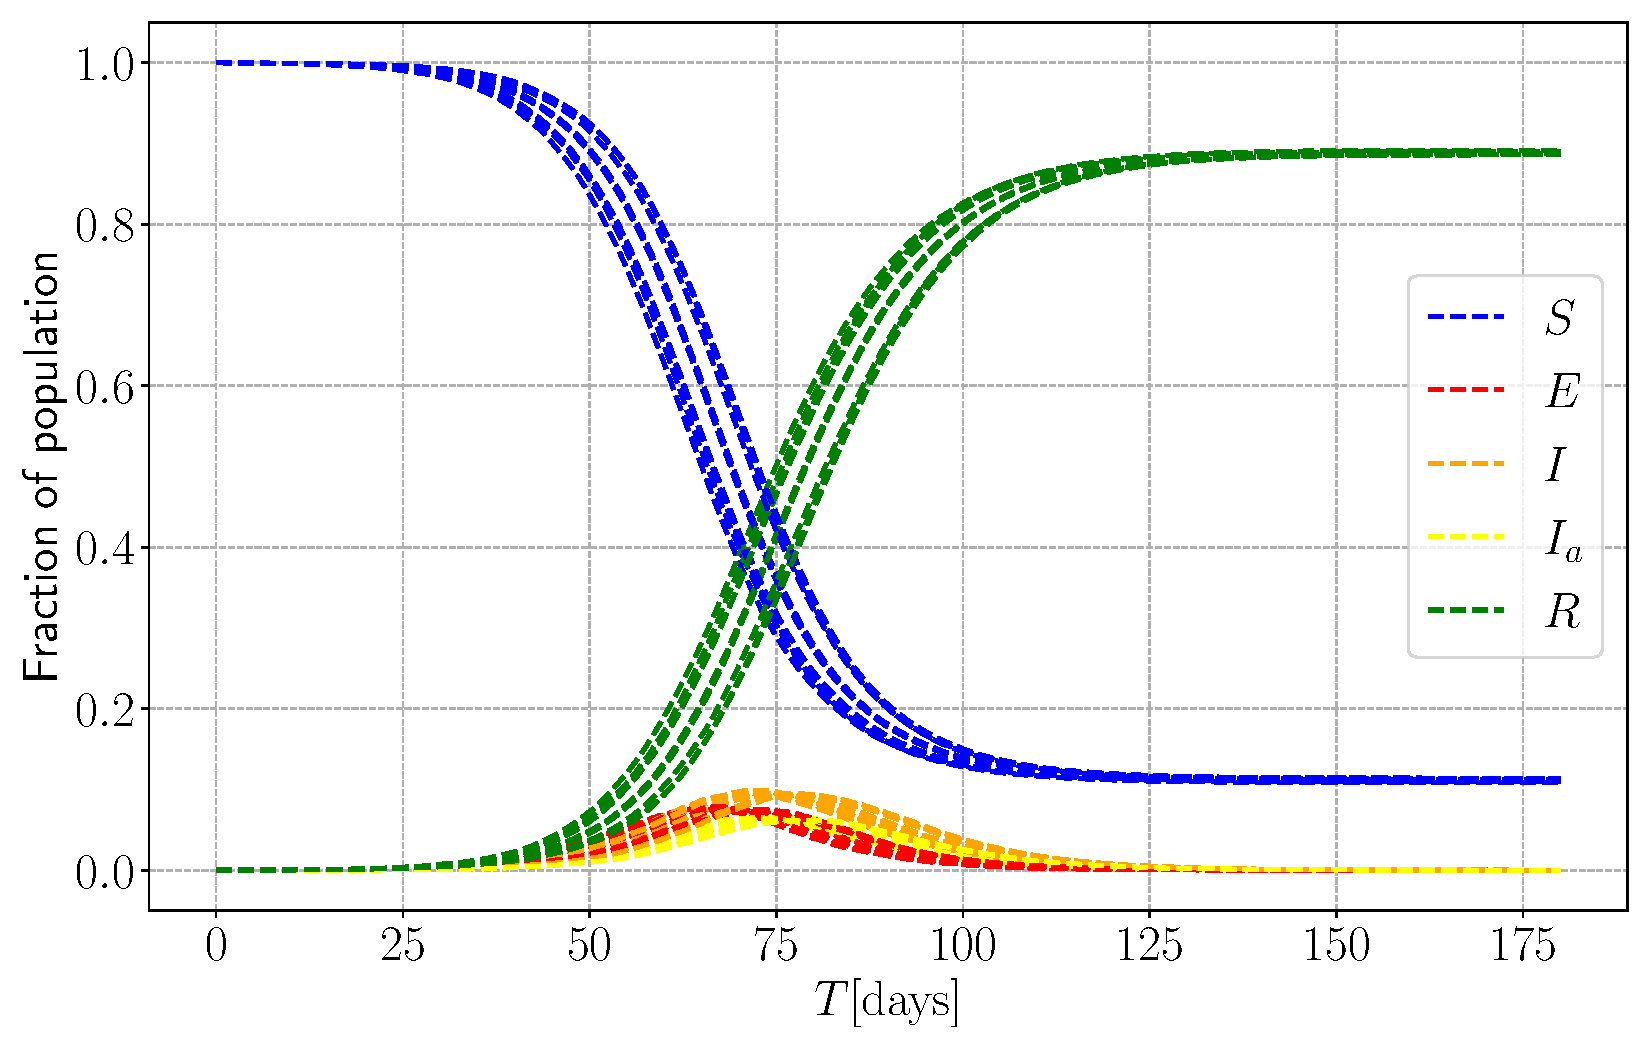
\includegraphics[width=0.8\columnwidth]{../fig/2Ca_SEIIaR.pdf}
	\caption{Solution of the stochastic SEIIaR-equations.}
	\label{fig:SEIIaR}
\end{figure}

\begin{figure}[htb]
	\centering
	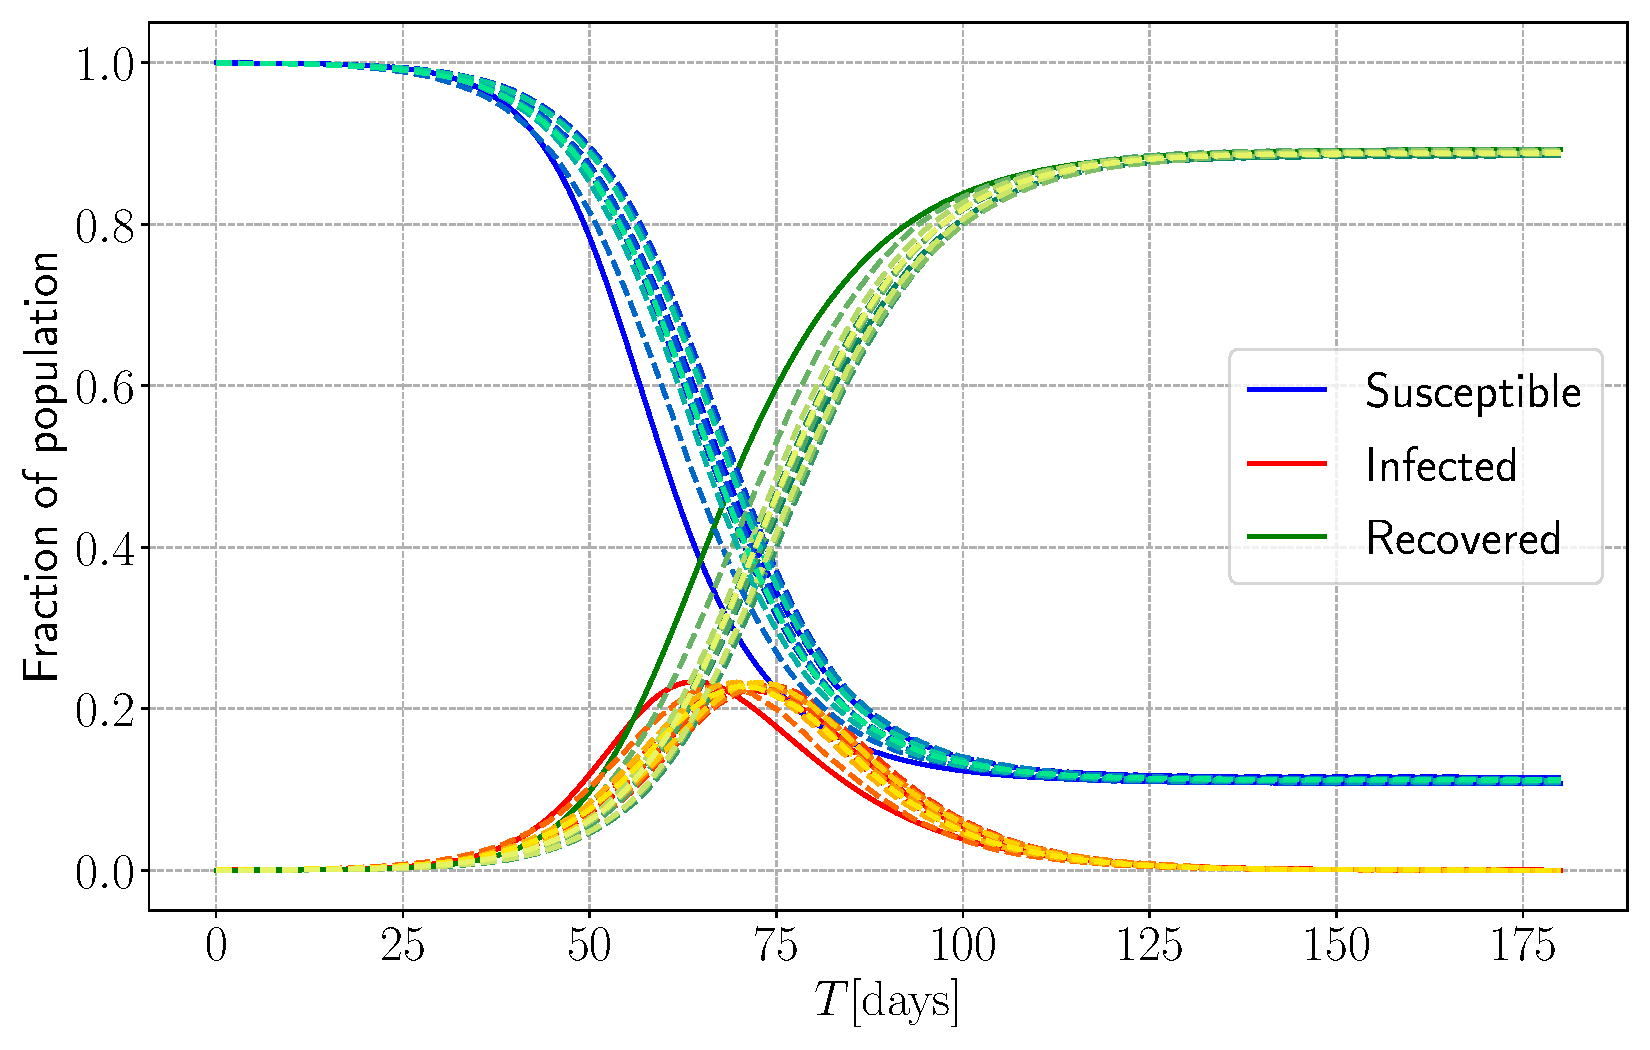
\includegraphics[width=0.8\columnwidth]{../fig/2Ca_comp.pdf}
	\caption{Comparison of the solution of the Stochastic SEIIaR-equations with the deterministic SIR-model. The number of infected people $I$ in the stochastic model is $E + I + I_a$.}
	\label{fig:SEIIaR_compare}
\end{figure}

One conspicuous feature to notice here, is that the process overall seems to be \textit{slower}, in the sense that it takes longer time for people to get infected and eventually recover, but the asymptotic behaviours seem to align quite closely. This is probably due to the fact that this model includes a period in which people are infected but not yet able to infect anybody else: an incubation period of typical length $\tau_E = 3 \, \mathrm{days}$. This will naturally delay the process, but it should not affect the asymptotic behaviour. The peak of the infected fraction is also seen to be slightly lower. This is also a result of this delay period making the infections more spread out in time. Ultimately, this shows that the SEIIaR model is more realistic in the sense that people do not get sick right away, and that the behaviour agrees with our expectations. Another thing to mention is that the fraction of infected asymptomatic people $I_a$ are always less than the fraction of infected symptomatic people $I$. This is as expected since $f_a < f_s$ and $r_a < r_s$.

To test that the implementation is correct --- by comparing with the deterministic and stochastic SIR model --- we adjust the parameters of the SEIIaR to $\beta = 0.25$, $r_s = 1$, $r_a = 1$, $\tau_E = 0$, $\tau_I= 10$ and start with $10$ out of $100 \, 000$ people initially infected. The results of doing $1000$ such simulations and performing the average of the stochastic models is shown in figure \ref{fig:comparison_SIR}. This shows that the two stochastic models are very similar, as expected. Furthermore we see that there seems to be a slight delay of the (mean of the) stochastic models compared to the deterministic one. This is however as expected, since only in the limit of $\Delta t\to 0$ \textit{and (crucially)} $N\to \infty$ does the stochastic SIR model coincide with the deterministic one, as discussed in the introduction in section \ref{sec:stochsirtheory}. Since we use populations of size $N = 10^5$ we must naturally expect such a deviation, despite the fact that we are using a \textit{small} time step and take the average of many simulations. This also emphasises the fact that using the deterministic model as a reference solution for determining the step length for the stochastic model(s) is probably not a good idea, since we don't even expect them to be equal when $\Delta t \to 0$, for finite $N$. 
%Furthermore, we also see that the overall process seems slightly delayed for the stochastic models compared to the deterministic. I am not quite sure what causes this, but I suspect that it might have something to do with the deterministic model, we can use the value of $\mathbf{f}$ in equation \eqref{eq:sir_vect} at times in between $t$ and $t+\Delta t$ to compute the value of $\mathbf{v}$, whereas the stochastic model only resolves time modulo intervals of length $\Delta t$.

\begin{figure}[h!]
	\centering
	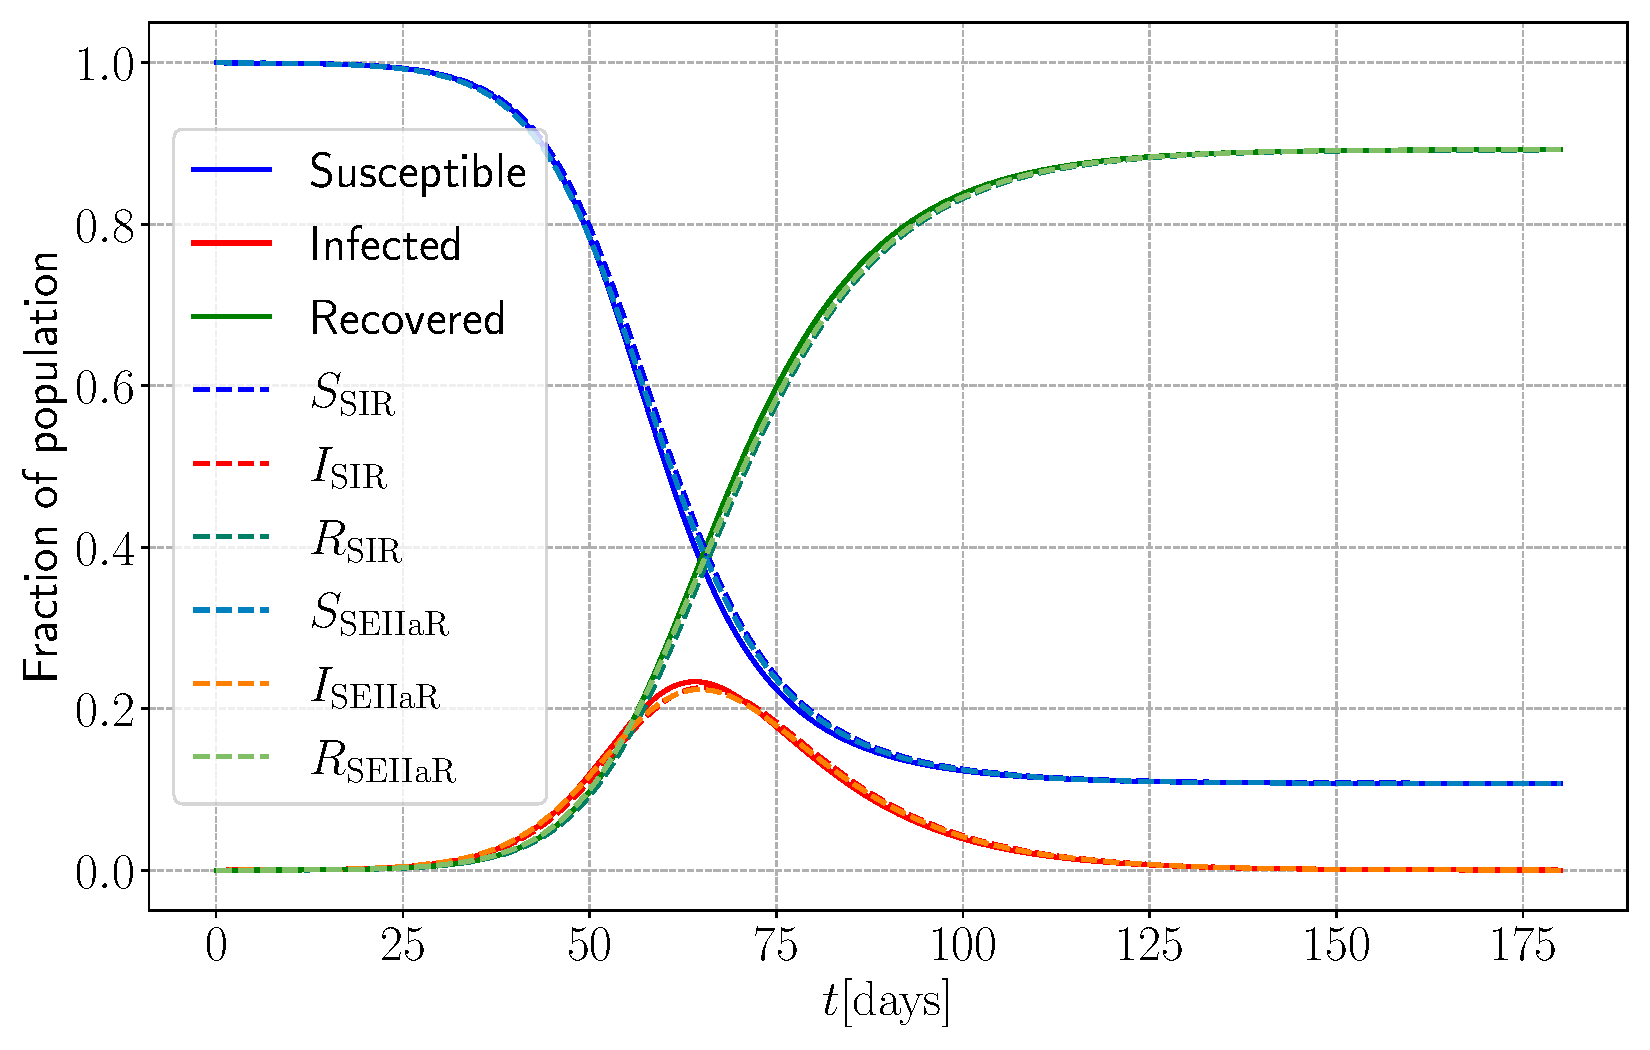
\includegraphics[width=0.8\columnwidth]{../fig/test_comparison.pdf}
	\caption{Solution of the stochastic SEIIaR-equations compared with the stochastic and deterministic SIR-equations for the case of identical parameters.}
	\label{fig:comparison_SIR}
\end{figure}
\newpage

\subsection{b) Probability of outbreak dependence on $r_s$}

The variable $r_s$ describes how infectious a person is when he is in the infected state. Reducing this constant below $1$ can therefore correspond to increasing the degree of self-isolation when people are symptomatic. We investigate the probability of an outbreak as a function of this self-isolation-rate $r_s$ by the following procedure (which is essentially the same as that shown in $2Bb$ expect we are now finding the probability as a function of $r_s$): 

\begin{algorithm}[H]
	Choose the parameters of the model as those given in the exam sheet \cite{sheet}, but with $T = 30 \, \mathrm{days}$\footnote{As the typical infection time is still $10$ days, I assume 30 days to be more than sufficient for detecting an outbreak in the stochastic model.}. \;
	Choose a batch-size $B$.\;
	Choose $n$ number of values of $r_s$ to try\;
	Select $n$ values of $r_s$, equally spaced between $0.001$ and $1$ :
		$$
			\mathbf{R} = [R_1, \dots R_n]
		$$
	\For{$i = 1,2,\dots, n$}{
		Initialise an empty vector of length $B$: $\mathbf{X} = [0,\dots,0]$.\;
		\For{$n = 1,\dots, B$}
		{
			Run the simulation with $r_s = R_i$.\;
			Calculate the \texttt{slope} in the semi-log axes for $I(t)$.\;
			\eIf{$\texttt{slope} <= 0$}
			{$X_n = 0$}
			{$X_n = 1$}
		}
		Estimate the probability of an outbreak when $r_s = R_i$ by
		$$
		p \coloneqq P(\mathrm{outbreak}|r_s) = \frac{1}{B} \sum_{n= 1}^{B} X_n. \;
		$$	
		Calculate the standard deviation of the estimate by 
		$$
		\sqrt{\mathrm{Var}(\hat{p})} = \sqrt{\frac{p(1-p)}{B}}.
		$$
	}
	\caption{Calculating the probability of an outbreak as a function of $r_s$.}
\end{algorithm} 

The results of this calculation using a batch size of $B = 500$ and $100$ values of $r_s$ are shown in figure \ref{fig:rs_prob}. The behaviour is as expected: when people are hardly infectious when symptomatic the probability of an outbreak is close to $0$. This is also probably also a result of the fact that $r_a = 0.1$, i.e. it is not particularly likely to infect anyone when you are asymptomatic. If $r_a$ and $f_a$ was higher, one would expect the probability distribution to stagnate at some finite value when $r_s \to 0$, or at least go to $0$ slower. This is demonstrated in the same figure, where we set $r_a = 1$ and perform the same test as above. This again is an intuitive confirmation that the model behaves as expected, and therefore is correctly implemented.

We see from this plot that an outbreak is almost certain to \textit{not} grow exponentially when $r_s \lesssim 0.2$, and for $r_s \simeq 0.38$ there is a probability of $0.46 \pm 0.022$ for an outbreak growing. 

\begin{figure}[htb]
	\centering
	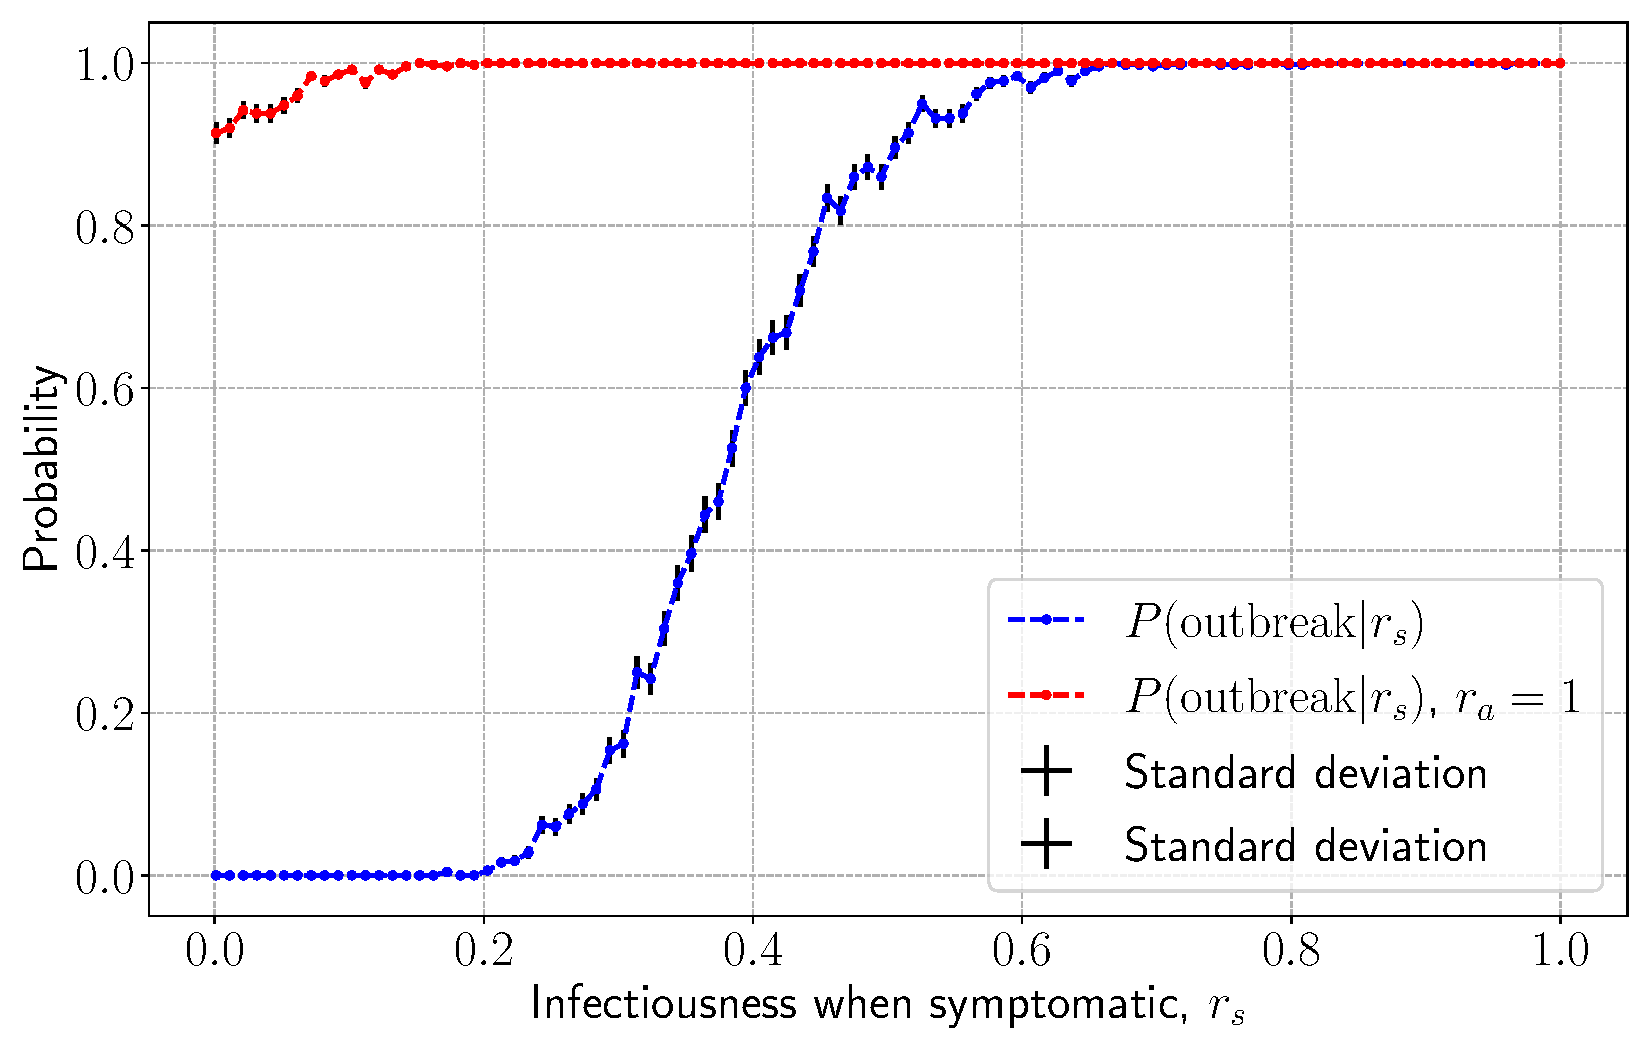
\includegraphics[width=0.8\columnwidth]{../fig/2Cb_probs.pdf}
	\caption{Probability of an outbreak as a function of $r_s$.}
	\label{fig:rs_prob}
\end{figure}


\clearpage